\section{Theoretical Work}

Our approach to speedup the algorithm is to simulate the changes that occur to matrix $Q$ during the algorithm in a data structure which handles the queries in polylogarithmic time. The desired data structure should capture changes to $Q$ after each step while maintaining the minimum element in $Q$ for the next step. We can use the minimum element in $Q$ to merge two taxa, and make queries to perform the induced changes in $Q$. We breakdown the required updates to capture all changes in $Q$, and show all except one of them can be performed on a $(2t-1) \times (2t-1)$ two-dimensional segment tree in polylogarithmic time. Our goal is to handle all updates in each step with a total of $\widetilde{O}(n)$ running time, while the number of updates in each step is $O(n)$.

\emph{Segment Tree} is a useful data structure to implement range queries and updates. It is a binary tree with $n$ leaves, where each node represents an interval on a sequence of length $n$. The root of this tree represents interval $[1, n]$, and a node representing interval $[l, r]$, for $l < r$, has two children representing $[l, (r + l) / 2]$ and $[(l + r) / 2 + 1, r]$. This way, the $i$-th leaf represents interval $[i, i]$. In this data structure, we can perform range updates and range queries in logarithmic time. For example, a range update $(l, r, v)$ adds a constant value $v$ to elements $l, l+1, \ldots, r$, and a range query $(l, r)$ returns the sum of elements $l, l+1, \ldots, r$. The main intuition for performing these updates and queries efficiently is that any given range $[l, r]$ can be decomposed into $O(\log{n})$ segment tree intervals. This process is illustrated in Figure \ref{segment-tree}.\footnote{For more details, take a look at \href{https://en.wikipedia.org/wiki/Segment_tree}{https://en.wikipedia.org/wiki/Segment\_tree}.}

\begin{figure}[h!]\label{segment-tree}
	\caption{An example of segment tree with some range queries decomposed into segment tree intervals (green labels above the nodes show the decomposition)}
	\begin{center}
		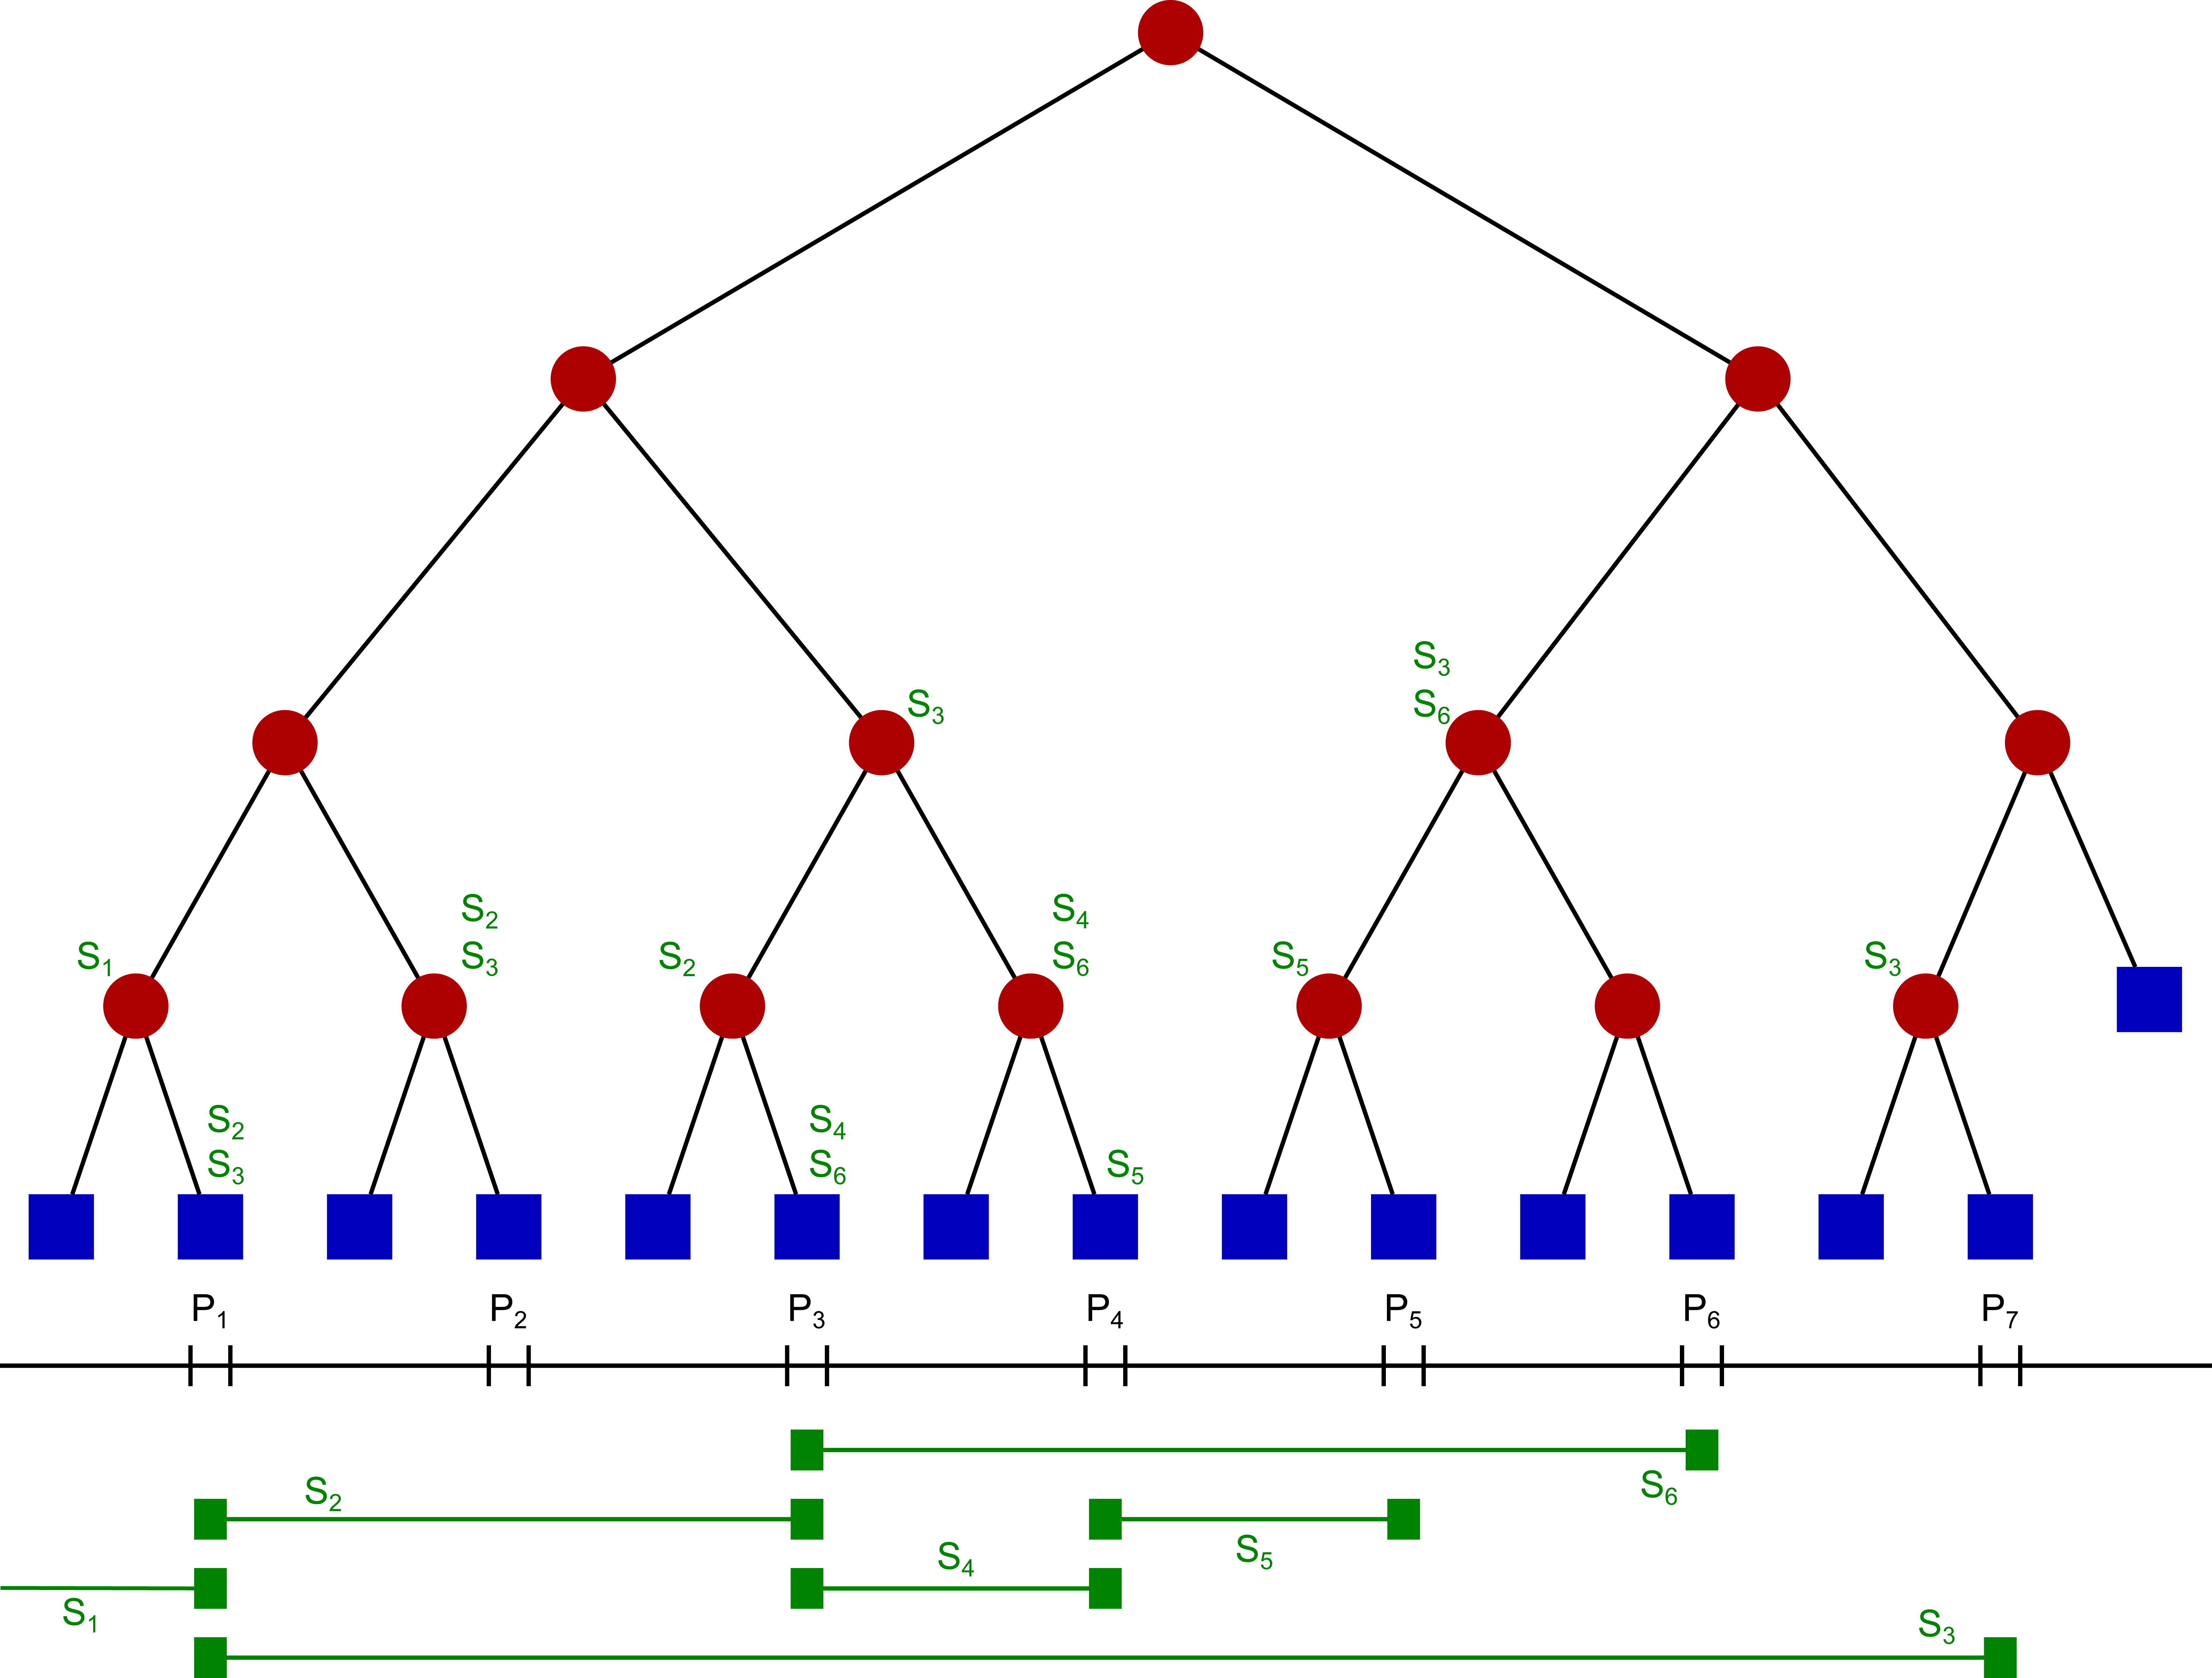
\includegraphics[width=8cm]{Segment_tree.png}
	\end{center}
\end{figure}

One can extend the notion of segment tree into higher dimensions, say a $d$-dimensional segment tree, by simply creating a one-dimensional segment tree of $(d-1)$-dimensional segment trees.  For the two-dimensional case, we create a one-dimensional segment tree by $x$-axis where each of its nodes contain a one-dimensional segment tree by $y$-axis. This results in $O(n^{d-1}\log{n})$ running time for submatrix queries and updates. Ibtehaz et. al~\cite{ibtehaz2018multidimensional} showed it is possible to implement a multi-dimensional segment tree capable of handling submatrix queries and updates in $O(\log{n}^d)$ time. We can use this result to perform polylogarithmic submatrix updates in our two-dimensional segment tree.

We can break down changes induced on $Q$ after each step as different submatrix queries. Recall equation \ref{qformula} for computing $Q(i,j)$:


\[Q(i,j) = (n-2)d(i,j) -\sum_{k=1}^n d(i,k) - \sum_{k=1}^n d(j,k).\]


At each step, we choose two taxa $i$ and $j$ with minimum $Q(i, j)$ to join. Next, we replace vertices $i$ and $j$ with a dummy new vertex labeled $u$. 

[TBD]